\chapter{序論}
\label{chap:introduction}

\section{背景}
\label{section:background}

組み込み向けデバイスの性能向上と低価格化により、身の回りの家具や家電をはじめとしたあらゆるものが
インターネットに接続し、協調して動作することで生活を豊かにするInternet of Things(IoT)が
普及しつつある。

Espressif Systemsによって開発されたESP32\cite{esp32}は、組み込み向けデバイスの中でも
比較的高性能かつ廉価なSoCの一つである。

\begin{itemize}
  \item Xtensa single-/dual-core 32-bit LX6 microprocessor(s), up to 600 MIPS
  \item 448 KB ROM, 536 KB SRAM
  \item 802.11 b/g/n
  \item Compliant with Bluetooth v4.2 BR/EDR and BLE specifications
\end{itemize}

ESP32は豊富な計算資源と高度な無線接続機能を提供する一方で、ESP32が搭載している
Xtensaマイクロプロセッサが用いるXtensa命令セットアーキテクチャ\cite{xtensa_isa}は、
幅広い開発環境にサポートされているとは言えない。
現在、ESP32向けのソフトウェア開発環境としてEspressif Systemsにより公式に提供されているのは、
以下の2通りの手段である\cite{esp_toolchain}。

\begin{itemize}
  \item C/C++でプログラムを記述し、ESP32 Toolchainによりコンパイルする
  \item Arduino言語でプログラムを記述し、Arduino IDEと
        Arduino core for ESP32 WiFi chipによりコンパイルする
\end{itemize}

x86やARMといった、広く利用されている命令セットアーキテクチャを搭載するPCやサーバ向けの
ソフトウェア開発では、開発者には多くの開発環境を選択肢として選択できる。
例えばプログラミング言語の選択という観点では、LLVMが機械語生成の対象としてサポートされている
ハードウェアであれば、LLVMを機械語生成に用いるプログラミング言語の全てが選択肢となりうる。
しかし、組み込み向けマイクロコントローラなど、用途が限定されているアーキテクチャの中でサポート
されているものは限られている\cite{llvm_matrix}。
Xtensaアーキテクチャも、LLVMによってサポートされていないものの一つである。

\section{本研究が着目する課題}

本研究では、\ref{section:background}節で述べた、ESP32向けのソフトウェア開発環境が
限られている点に着目する。
多くの開発環境でサポートされているアーキテクチャをESP32上で実行することができれば、
ESP32に向けたソフトウェア開発環境の選択肢を広げることができる。

\section{本研究の目的とアプローチ}

本研究の目的は、Xtensaアーキテクチャよりも多くの開発環境でサポートされているアーキテクチャ
向けにコンパイルされたプログラムを、ESP32上で実行することである。

そこで、本研究では仮想命令セットアーキテクチャとしてWebAssemblyを用いることを提案する。
また、実行形式としてWebAssemblyバイナリフォーマットを用いることを提案する。

本研究では、WebAssembly実行環境をESP32上に実装し、汎用的な開発環境を用いて生成された
プログラムを実行できることを示す。
これにより、仮想命令セットアーキテクチャとしてWebAssemblyを用いることで、ESP32の開発環境の
選択肢を広げられることを示す。

\begin{figure}[htbp]
  \caption{現状と展望}
  \label{fig:new_world}
  \begin{center}
    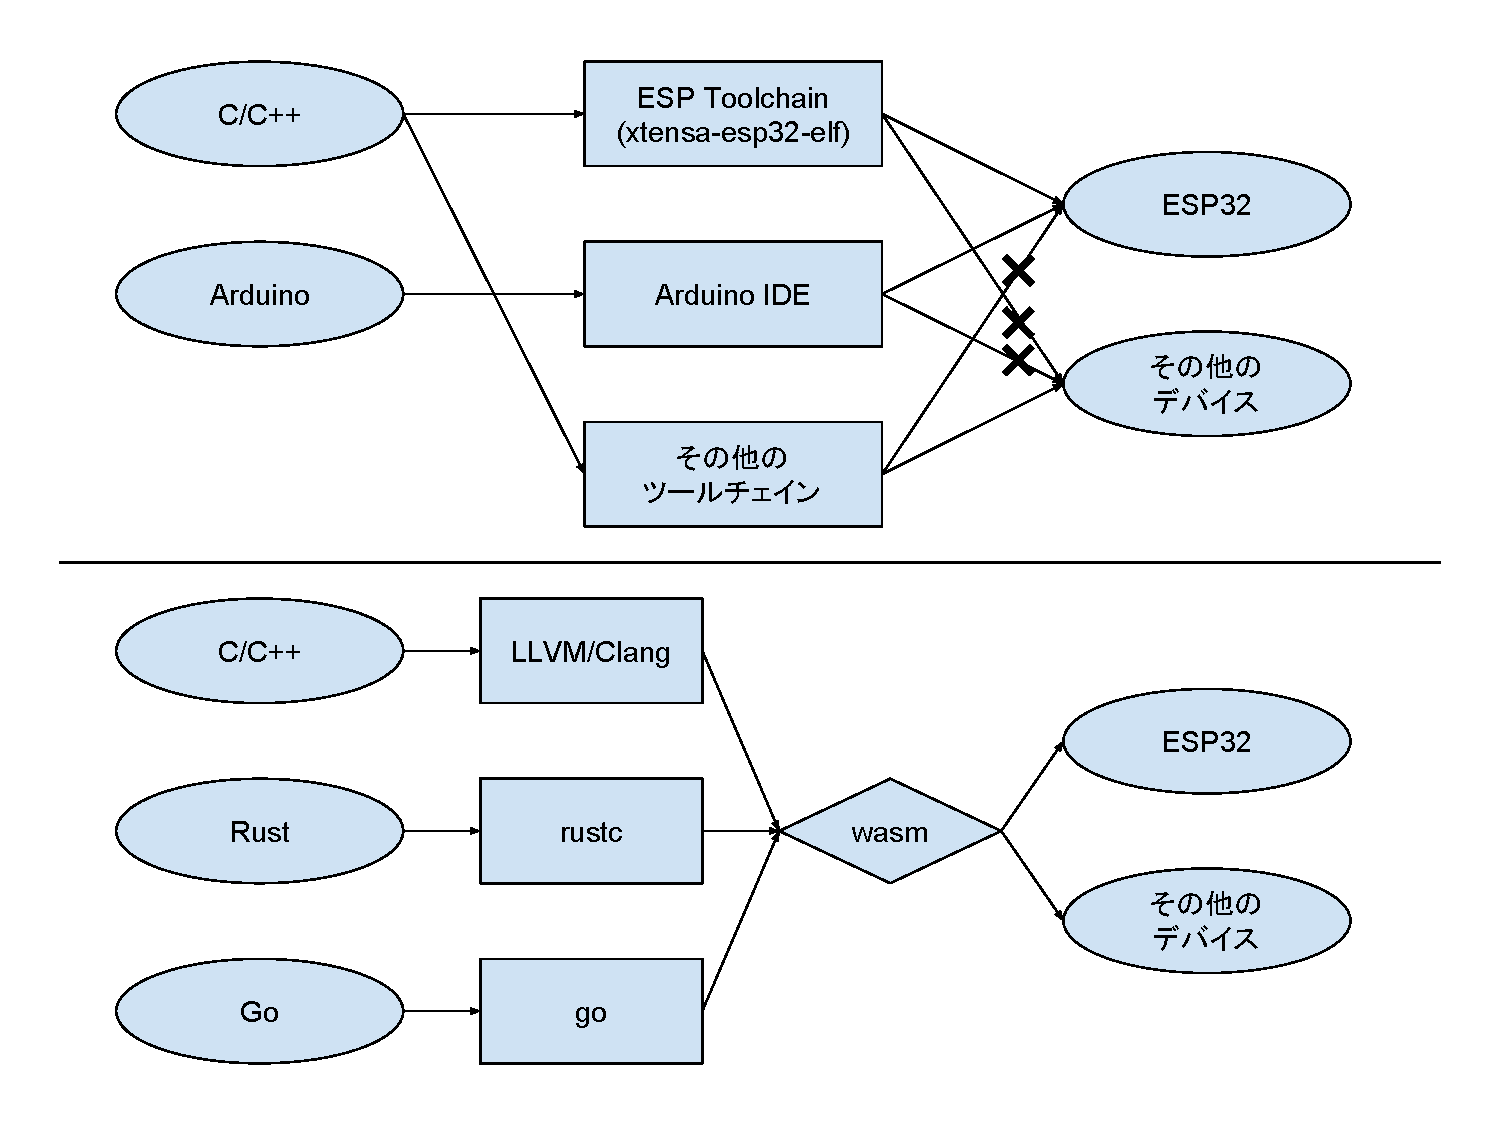
\includegraphics[bb=0 0 800 600,width=12cm]{img/new_world.pdf}
  \end{center}
\end{figure}

\section{本研究の構成}

本論文における以降の構成は次の通りである。

\ref{chap:related_works}章では、関連技術として〜。
\ref{chap:implementation}章では、本研究で実装するWebAssembly実行環境について、
設計と実装を示す。
\ref{chap:evaluation}章では、〜。
\ref{chap:conclusion}章では、〜。
